\begin{chapter}[beamerthemesrc/assets/background_negative]{}{Interprétation, Compilation \& Mémoire}
    \begin{itemize}
          \item Interprétation \& Compilation des langages
          \item Tas \& Pile
          \item Table des symbôles
    \end{itemize}
\end{chapter}

\begin{frame}{Interprétation \& Compilation}
    \begin{block}{}
        \begin{itemize}
            \item Utilisation du patron de conception \textbf{Visiteur}
            \item Application des règles d'interprétation MiniJaja \& JajaCode
        \end{itemize}
    \end{block}
    \begin{figure}
        \centering
        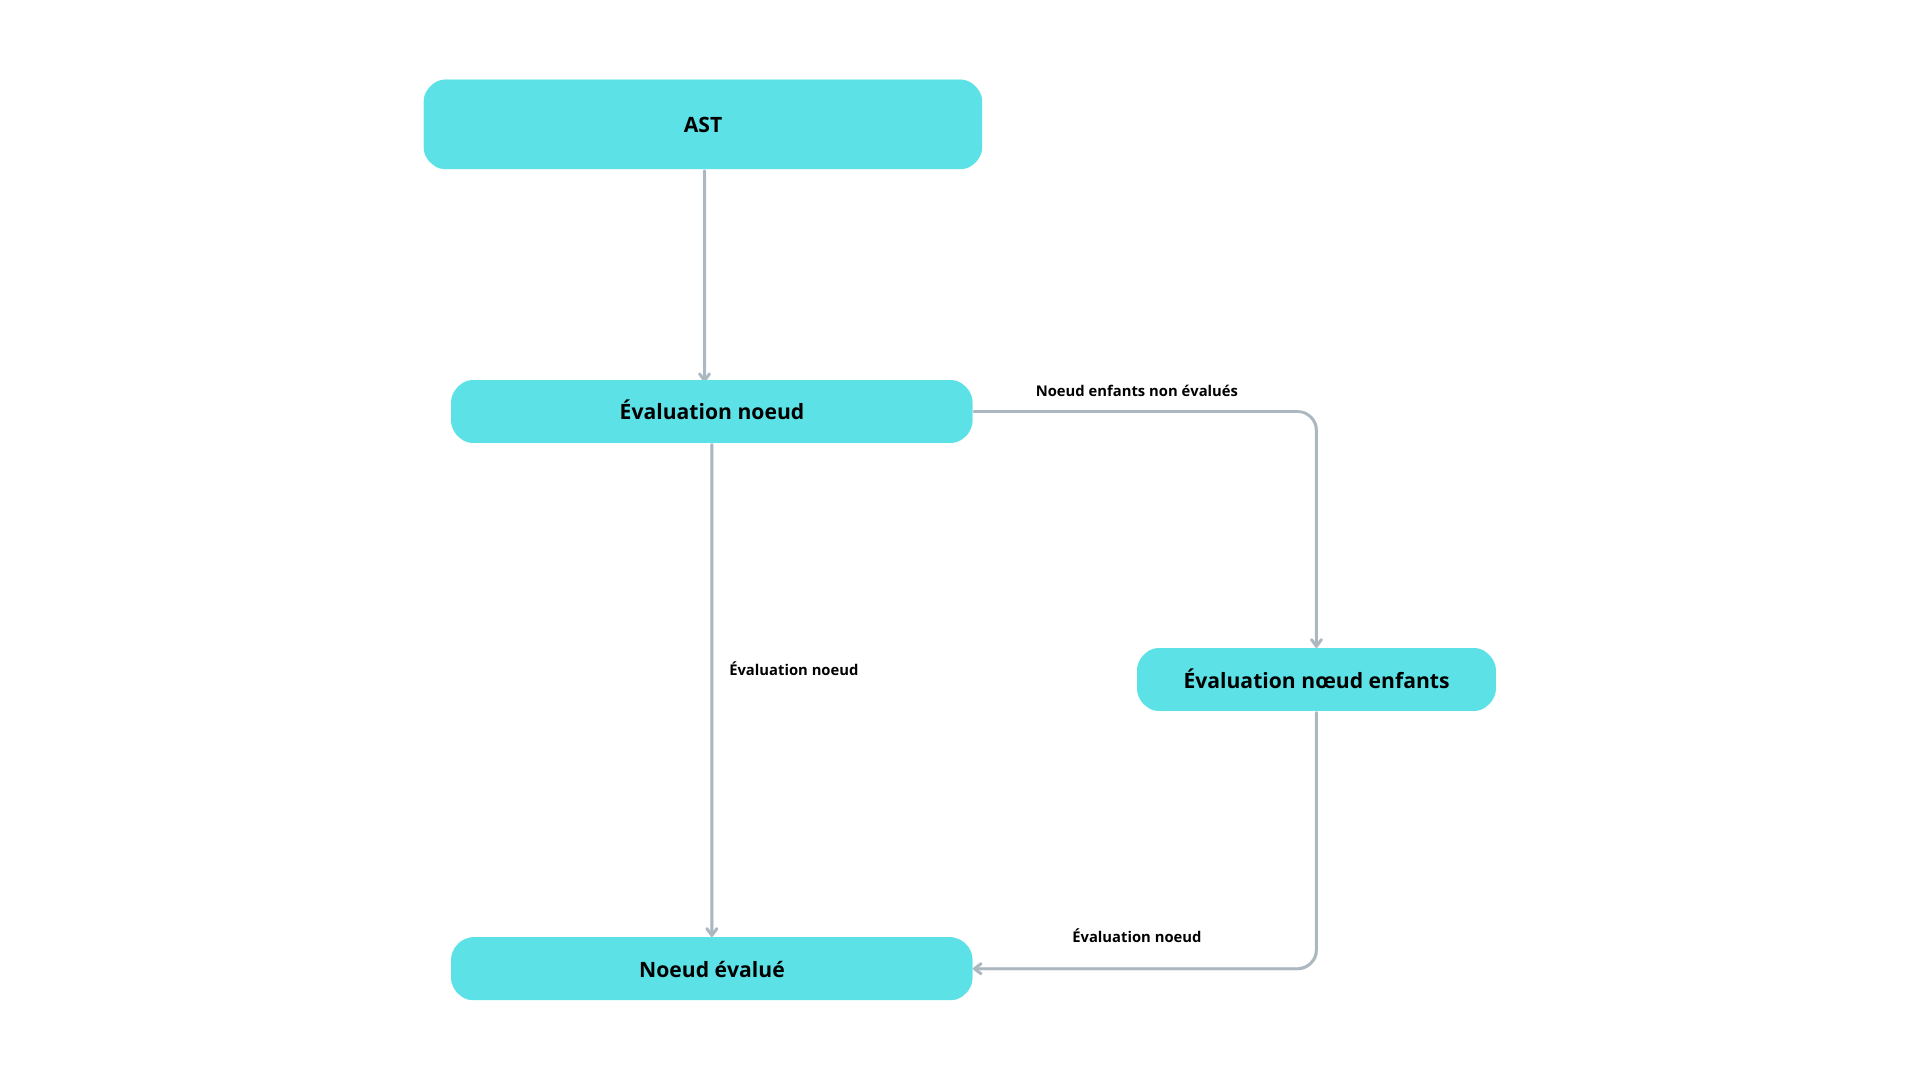
\includegraphics[width=0.5\textwidth]{contents/images/jjtAccept.png}
    \end{figure}
\end{frame}

\begin{frame}{Tas \& Pile}
    \begin{block}{Tas}
        \begin{itemize}
            \item Diviser en bloc de puissance de 2
            \item Découper au plus juste
            \item Agrandir la taille du tas si nécéssaire
            \item Reconstruire le tas avec stratégie
        \end{itemize}
    \end{block}

    \begin{block}{Pile}
        \begin{itemize}
            \item Fonctionnel comme une pile classique
            \item Favorable au stockage des objets mémoire
            \item Essentiel pour le bon fonctionnement du programme
        \end{itemize}
    \end{block}
\end{frame}

\begin{frame}{Table des symbôles}
    \begin{block}{}
        \begin{itemize}
            \item Fonctionnement en pile
            \item Association de chaque portée à une table de hachage
            \item Retrait de la table des symboles à la fin de la portée
        \end{itemize}
    \end{block}
\end{frame}
